\subsubsection{Mathematical Modeling of Marine-related Exchange Processes}
\index{Khalili, Arzhang}

%________________________

\paragraph{Research Team}
%________________________

Arzhang Khalili (Professor), Meheboob Alam (Visiting Professor),
Somnath Bhattacharyya (Visiting Professor),
Karsten Lettmann (Postdoctoral Student), Guohui Hu (Visiting Professor),
Bo Liu (Postdoctoral Student)

\medskip

The main research topics were the use and improvement of numerical
techniques and hydrodynamic stability analysis for mathematical modeling of
    flow through sinking aggregates
        (with Prof. S. Bhattacharyya,
        Indian Institute of Technology, Kharagpur, India),
    for instability studies on granular layers by viscous shear flow
        (with Prof.~M. Alam, Jawahar-Nehru-Center for
        Applied Scientific Research (JNCASR),
    for modeling sediment transport
        (with B. Liu),
    and for the development of a diagenesis
    simulation code for marine sediments
        (with K. Lettmann)

%_____________________

\paragraph{Highlights}
%_____________________

Marine aggregates are known as medium of transport of food
and energy from the surface water of seas and oceans down to the seabeds.
Marine scientists are interested in estimating the release or absorption
of nutrients from the aggregates into the seawater or vice versa.
The distribution of the nutrient release/absorption is a complex phenomenon
which can only be studied using mathematical simulations.
The present models in the literature (for example, Ki{\o}rboe et al.\ 2001)
depart from a solid sphere as the aggregate geometry.
Transmission electron microscopy images shows that marine aggregates have
a porous structure. Therefore, we developed a mathematical
\cite{BhaDhiKha06} method to account
for the simulation of flow and concentration field through and around
sinking marine aggregates (see Fig.~\ref{fig:kahlili-fig}).

\begin{figure}[ht]
  \begin{center}
    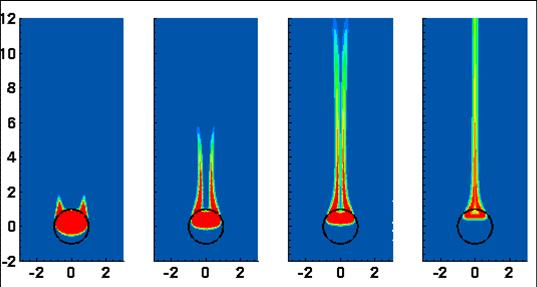
\includegraphics[width=\hsize]{Khalli/khalili-fig.jpg}
    \mycaption{The removal of nutrients from
        sinking marine aggregates as
        a function of time}
    \label{fig:kahlili-fig}
   \end{center}
\end{figure}

Further, a Lattice Boltzmann Formulation of an aggregate composed
of an ensemble of smaller particles has already been investigated
\cite{BhaKha06}.

At the moment we try to bring more insight into this problem using
the non-invasive visualization method `positron emission tomography'
(PET).


Another research topic was the formation of granular beds under the
effect of shear flows.
It is known that a sand-bed can deform into several types of
configurations when a fluid (water or air) flows over it.
Depending on the strength of the flow and the properties of the
bed-material, the nature of interaction between the bed and the
fluid will vary which, in turn, decides the resulting
pattern formation over the bed.
Though many studies have been discussing this issue,
the phenomenon has not been yet properly understood.
A new set of fundamental equations for description of
flow of granular media are jointly with Prof.~M. Alam (JNCASR)
being developed at the moment.
We are developing a new particle dynamics model to address this
question. A manuscript is submitted.

Within a project with a former postdoctoral student, the
hydrodynamic instability of a flow within a porous channel
was also successfully studied \cite{BerKha06}.

Due to the relevance of gas migration from the sea bottom
and its role for understanding the global methane
turnover, an experimental study was made to understand the
mechanisms of buoyancy-affected gas migration in
unconsolidated porous media \cite{StoKha06}.


An emphasis of the research in 2006 was also put on the development of a
dynamic model for sulfate-methane with single/double
organic carbon decay rate/s.
Our present model can be considered as a static model without
the influence of the advection. In the next step, the dissolved
and gaseous methane as well as organic carbon should be
spatially distributed by the existence of an advective flow.
Such a model is a very useful tool to understand, for example, the
process of organic matter oxidation in seas. A major part of the model
has been already developed.
This work is to be continued.

In 2006, and certainly 2007, sediment transport will be an
important aspect of my work.
Complex fluids in the form of liquids with solid particles suspended in
them are significant in many fields of industry as well as in
biological processes and in nature.
Several methods have been developed to simulate the suspension
flows. So far the largest and maybe the most realistic
suspension simulations have been performed with the
Lattice-Boltzmann method that appears to be efficient
for simulating various multi-phase-flow problems.

The simulation can describe the erosion of a synthetic fracture and incorporate the explicit topography of the pore space; the transport coefficients are determined independently.


%_______________________

\paragraph{Organization}
%_______________________


\begin{enumerate}
\item  Meetings: DFG-Graduiertenkolleg, \\ PoreNet, Faculty 4,
    University Bremen
\item  International Workshop on Marine Aggregates (IWOMA),
       December, 11--12, 2006
\end{enumerate}

%_______________________

\paragraph{Collaborations}
%_______________________

\begin{enumerate}
\item {\sl Jawahar-Nehru-Center, India} \\ Prof.~M.~Alam \\
    Instabilities of granular beds under shear flows
\item {\sl Massachusetts Institute of Technology, USA} \\
    Prof.~C. C. Mei \\
    Wave effects on formation of beds
\item {\sl Texas A\&M University, USA} \\ Prof.~G. Jackson \\ Marine Aggregates
\item {\sl Danish Institute for Fisheries Research} \\
    Prof.~T. Ki{\o}rboe \\ Marine Aggregates
\item {\sl Scripps Institution of Oceanography}       \\
    F.~Azam \\ Marine Aggregates

\end{enumerate}

%_________________

\paragraph{Grants}
%_________________
% list the running grants in 2006, if none have been received, please delete this
% subsection.
\begin{enumerate}

\item Funded by Max Planck Society, \emph{Erosion of granular
beds}, (2007--2010) \item Funded by DFG, \emph{Modeling and
visualization of flow in porous
      media}, (2006--2008)
\item Funded by DFG, \emph{3D-flow through marine aggregates},
      (June--August 2006)
\item  Funded by HWK, \emph{Particle models for marine
aggregates},
      (September--November 2006)
\end{enumerate}

%_________________________

%\paragraph{Awards, Prizes}
%_________________________
%
% list the grants you have received in 2005, if none have been
% received, please delete this
% subsection.
%\begin{enumerate}
%\end{enumerate}
